\lhead{\emph{Dominio del problema}}
\chapter{Dominio del problema}

La utilización de algoritmos distribuidos implica mejoras sustanciales en una gran cantidad de aplicaciones, incrementando la capacidad global de cómputo de un sistema mediante la unión de varios dispositivos que trabajan como una única unidad manteniendo simultáneamente un alto grado de independencia y una tolerancia global a fallos muy alta. Sin embargo, el coste de la adquisición instalación y mantenimiento de dicho conjunto de nodos suele ser elevado. Además, los beneficios citados implican una mayor complejidad en el desarrollo de algoritmos que puedan aprovechar de forma óptima este tipo de sistemas. Varios factores como la sincronización y la comunicación entre partes, o errores tales como condiciones de carrera son mucho más comunes que en otro tipo de aplicaciones. Dichas circunstancias no solo dificultan el desarrollo de este sistema, sino también la comprensión de los fundamentos básicos de la Computación Distribuida, aspecto de relevancia para estudiantes de Ciencias de la Computación.

Si bien la mayoría de las aplicaciones en las que el paradigma de computación distribuida introduce mejoras suelen exigir una gran capacidad de cálculo, su desarrollo únicamente requiere un conjunto de instancias independientes de un \textit{software} (sistema operativo, contenedor de servicios\dots) con las que trabajar. Dicha característica implica que la utilización de nodos de precio reducido (o incluso equipos ya presentes en una infraestructura) para el diseño, análisis y evaluación de este tipo de algoritmos constituye una alternativa válida frente a sistemas de precio superior.

Sumada a dicha motivación existe el potencial aprovechamiento de este sistema como herramienta didáctica que facilite el aprendizaje de conceptos como el reparto de procesos, balance de carga o la compartición de recursos en asignaturas centradas en este tipo de conceptos dentro de los planes de estudio de Ingeniería Informática o titulaciones similares.

En el presente proyecto se realiza un análisis de las diferentes alternativas que permitan satisfacer los objetivos definidos previamente.

%TODOFigura: Tabla de alternativas

\section{Definiciones}

\subsection{Definición del dominio del problema}

%TODO

\subsection{Sistema actual: Infraestructura de la Facultad de Ciencias}
\label{dominioproblema:infraestructura}
El sistema se ubica en una Facultad universitaria con 1.463 alumnos\cite{uecusal:estudiantes} en titulaciones relacionadas con las Ciencias de la Computación. Estas titulaciones cuentan con varias asignaturas relacionadas con el áreas de conocimiento Computación Distribuida, en particular \textbf{Arquitectura de Computadores} y \textbf{Sistemas Distribuidos} \cite{DIA15GuiaAcademica}. La Facultad cuenta con varias aulas y laboratorios de informática donde los alumnos disponen de la infraestructura necesaria para realizar los ejercicios y prácticas asignadas. Dichos espacios permiten utilizar cualquier equipo como nodo, pues se integran en la misma red, siendo incluso factible la comunicación directa entre equipos situados en diferentes aulas o incluso edificios. Todos los edificios cuentan con un cableado capaz de soportar teóricamente transferencias de hasta 100 Mb/s de forma bidireccional. La gestión de un sistema de autenticación se realiza mediante el protocolo \textbf{LDAP} (\textit{Lightweight Directory Access Protocol})\cite{RFC4516-comment}, contando con un sistema de ficheros centralizado que permite acceder a la información de un usuario desde cualquier equipo, facilitando las tareas de replicación de la información entre nodos\footnote{Datos extraídos de entrevistas con el Administrador de la infraestructura}.

La mayoría de las prácticas asignadas a los alumnos en las asignaturas de interés son desarrolladas en los lenguajes de programación \textbf{C} y \textbf{Java}, ya conocidos por la totalidad de los estudiantes gracias a asignaturas previamente cursadas.

\paragraph{Problemas conocidos}

Si bien la infraestructura existente es capaz de proveer a los estudiantes de los recursos necesarios, se identifican una serie de problemas inicialmente:

\begin{itemize}
  \item Cada grupo de alumnos necesita tres estaciones de trabajo para poder realizar algunos de los ejercicios propuestos.
  \item El servidor \textbf{LDAP} constituye un ``cuello de botella'', pues todos los alumnos acceden a él de forma intensiva, provocando el fallo por exceso de peticiones del mismo.
  %TODO\item Las técnicas de programación utilizadas hasta la fecha tienen un rendimiento bajo y son en ocasiones relativamente complejas.
\end{itemize}

\subsubsection{Análisis de estadísticas}
\label{dominio:estadisticast}
%Pandora magic

\section{Identificación de \textit{stakeholders}}

Un \textit{stakeholder} es cualquier grupo o individuo que tiene es afectado o afecta a la consecución de los objetivos de un proyecto marcados por una organización, así como un particular interés en el devenir del mismo. Claros ejemplos de este tipo de entidades son los diferentes usuarios finales del sistema, potenciales clientes o el equipo de desarrollo, entre muchos otros.

En el proyecto en cuestión se identifican los siguientes \textit{stakeholders} y su motivación.

\begin{itemize}
  \item Equipo de desarrollo. Su motivación es la consecución de todos los objetivos marcados en el sistema.
  \item Estudiantes de tercer y cuarto curso del Grado en Ingeniería Informática, que podrán utilizar el sistema como herramienta didáctica.
  \item Profesores de las asignaturas Arquitectura de Computadores y Sistemas Distribuidos, que aprovecharán el sistema final en dichas asignaturas.
  \item Administradores del sistema, que deberán hacerse cargo del mantenimiento del sistema a largo plazo.
\end{itemize}

\subsection{Identificación de las necesidades de cada parte}

Basándose en la motivación de cada parte es posible definir las demandas de cada una de las partes. Otros mecanismos, como la realización de entrevistas u observaciones permiten complementan dicho proceso.

\subsubsection{Alumnos}

\begin{itemize}
  \item Entorno de trabajo intuitivo y documentado que agilice el desarrollo de sus prácticas.
  \item Posibilidad de observar los resultados de las ejecuciones de forma sencilla.
  \item Depuración sencilla.
  \item Facilidades para el despliegue de los diferentes ejecutables en todas las máquinas, así como el consumo de los servicios que estos implementen.
\end{itemize}

\subsection{Necesidades de los docentes}

\begin{itemize}
  \item Entorno versátil sobre el cual puedan llevarse a cabo la totalidad de las prácticas y ejercicios propuestos, aportando si es posible algún tipo de ventaja sobre el sistema en uso.
  \item Instalación y configuración simple.
\end{itemize}

\subsection{Administradores}

\begin{itemize}
  \item Sistema integrable en la infraestructura actual cuyo mantenimiento sea sencillo y cuyo enfoque garantice la escalabilidad y su durabilidad. Documentación extensa sobre el funcionamiento interno del sistema.
  \item Instalación y configuración simple.
  \item Mantenimiento sencillo.
\end{itemize}

\section{Propuestas para la búsqueda de necesidades}

\begin{itemize}
  \item Encuestas o entrevistas a todas las partes.
  \item Observación.
  \item Evaluación de la experiencia de uso en las diferentes etapas de desarrollo del sistema.
\end{itemize}

\section{Identificación de requisitos}

\subsection{Requisitos de almacenamiento de la información}

\begin{itemize}
  \item Gestión de usuarios (credenciales de autenticación).
  \item Gestión de los datos de cada usuario.
  \item \textit{Logs} del sistema
  \item Ficheros de configuración, bases de datos de gestión\dots
\end{itemize}

\subsection{Identificación de requisitos funcionales}


\subsection{Identificación de requisitos no funcionales}

\subsubsection{Mantenimiento y robustez}

El \textit{software} debe ser mantenible y robusto, siendo dicha robustez garantizada mediante el uso de \textit{software} utilizado por una base de usuarios significativa, una arquitectura conocida, pruebas realizadas sobre él o un equipo de desarrollo en activo, entre otras.

\subsubsection{Costes de desarrollo}

El coste de desarrollo no debe superar un total de 400 €.

\subsubsection{Definición de los protocolos de comunicación}

Los diferentes protocolos utilizados o creados para el sistema deben ser públicos y extensibles a diferentes paradigmas de utilización y tecnologías que los implementen.

\subsubsection{Definición de los protocolos de seguridad y confidencialidad}

Se utilizará una infraestructura de clave pública para la mayoría de las transacciones cifradas realizadas en el sistema.

\subsubsection{Definición de la interacción con el usuario}

Todos los mecanismos de interacción con el usuario deberán definirse de forma precisa.

\subsubsection{Integridad del sistema y fiabilidad (\textit{uptime}, recuperación frente a fallos)}

\subsubsection{Compatibilidad con prácticas y otros ejercicios}

El sistema deberá ser compatible los ejercicios desarrollados en las asignaturas \textbf{Arquitectura de Computadores} y en especial \textbf{Sistemas distribuidos}

\section{Situación actual (\textit{state of the art})}
\label{stateoftheart}
En esta sección se definen diferentes enfoques ya aplicados a soluciones a problemas similares al planteado anteriormente.

\subsection{Computadores de placa única}

El uso de computadores de prestaciones reducidas como componentes de un sistema distribuido ha experimentado un gran crecimiento en los últimos años debido a la popularización y el abaratamiento de este tipo de dispositivos, existiendo gran cantidad de fabricantes y proveedores de \textit{software} para los mismos.

Los computadores de placa única (\textit{Single-Board Computers}) son máquinas de generalmente bajas prestaciones que aglutinan todos los componentes necesarios para su funcionamiento en un único circuito impreso. Suelen tener un coste bajo y una relación rendimiento/coste elevada. Su versatilidad y precio reducido han propiciado su uso como herramienta para el estudio y creación de sistemas distribuidos con un gran rango de propósitos diferentes.

\subsubsection{RPiCluster (Joshua Kiepert)}

Joshua Kiepert, estudiante de doctorado en la universidad Boise State, crea este sistema utilizando 33 computadores \textbf{Raspberry Pi B}, con el objetivo de utilizarlo como herramienta de pruebas que sirva de alternativa al supercomputador con el que su universidad cuenta\cite{joshuarpicluster} y sobre el que trabaja de forma rutinaria, con el objetivo de poder continuar su trabajo en periodos de mantenimiento, cierre del centro, etcétera. El sistema está diseñado para utilizar la \textit{Message Passing Interface} como mecanismo de comunicación y coordinación (siguiendo un esquema maestro-esclavo) y además utilizar los diferentes puertos de las placas (GPIO, I\textsuperscript{2}C, SPI, UART), puertos generalmente ausentes en computadores convencionales. Utiliza además un sistema \textbf{NFS} (\textit{Network File Storage}) para compartir datos entre todos los nodos, y un \textit{router} dedicado para la interconexión. El sistema se completa con un ordenador portátil \textbf{Chromebook} con el mismo sistema operativo que los nodos del sistema, (\textbf{Arch Linux}), que actúa como nodo coordinador. La estructura incluye el conjunto de nodos esclavos y coordinador, dos fuentes de alimentación y un mecanismo de refrigeración, así como un mecanismo de distribución de la energía (diseñado por Kiepert) y de gestión de los diodos LED que incluye cada nodo y que son utilizados como elemento estético y mecanismo de análisis visual del comportamiento de los algoritmos ejecutados\footnote{Vídeo del sistema en ejecución: \href{https://www.youtube.com/watch?v=i_r3z1jYHAc}{youtube.com/watch?v=i\_r3z1jYHAc}}.

%TODO: http://www.zdnet.com/article/build-your-own-supercomputer-out-of-raspberry-pi-boards/

\begin{figure}[H]
  \centering
  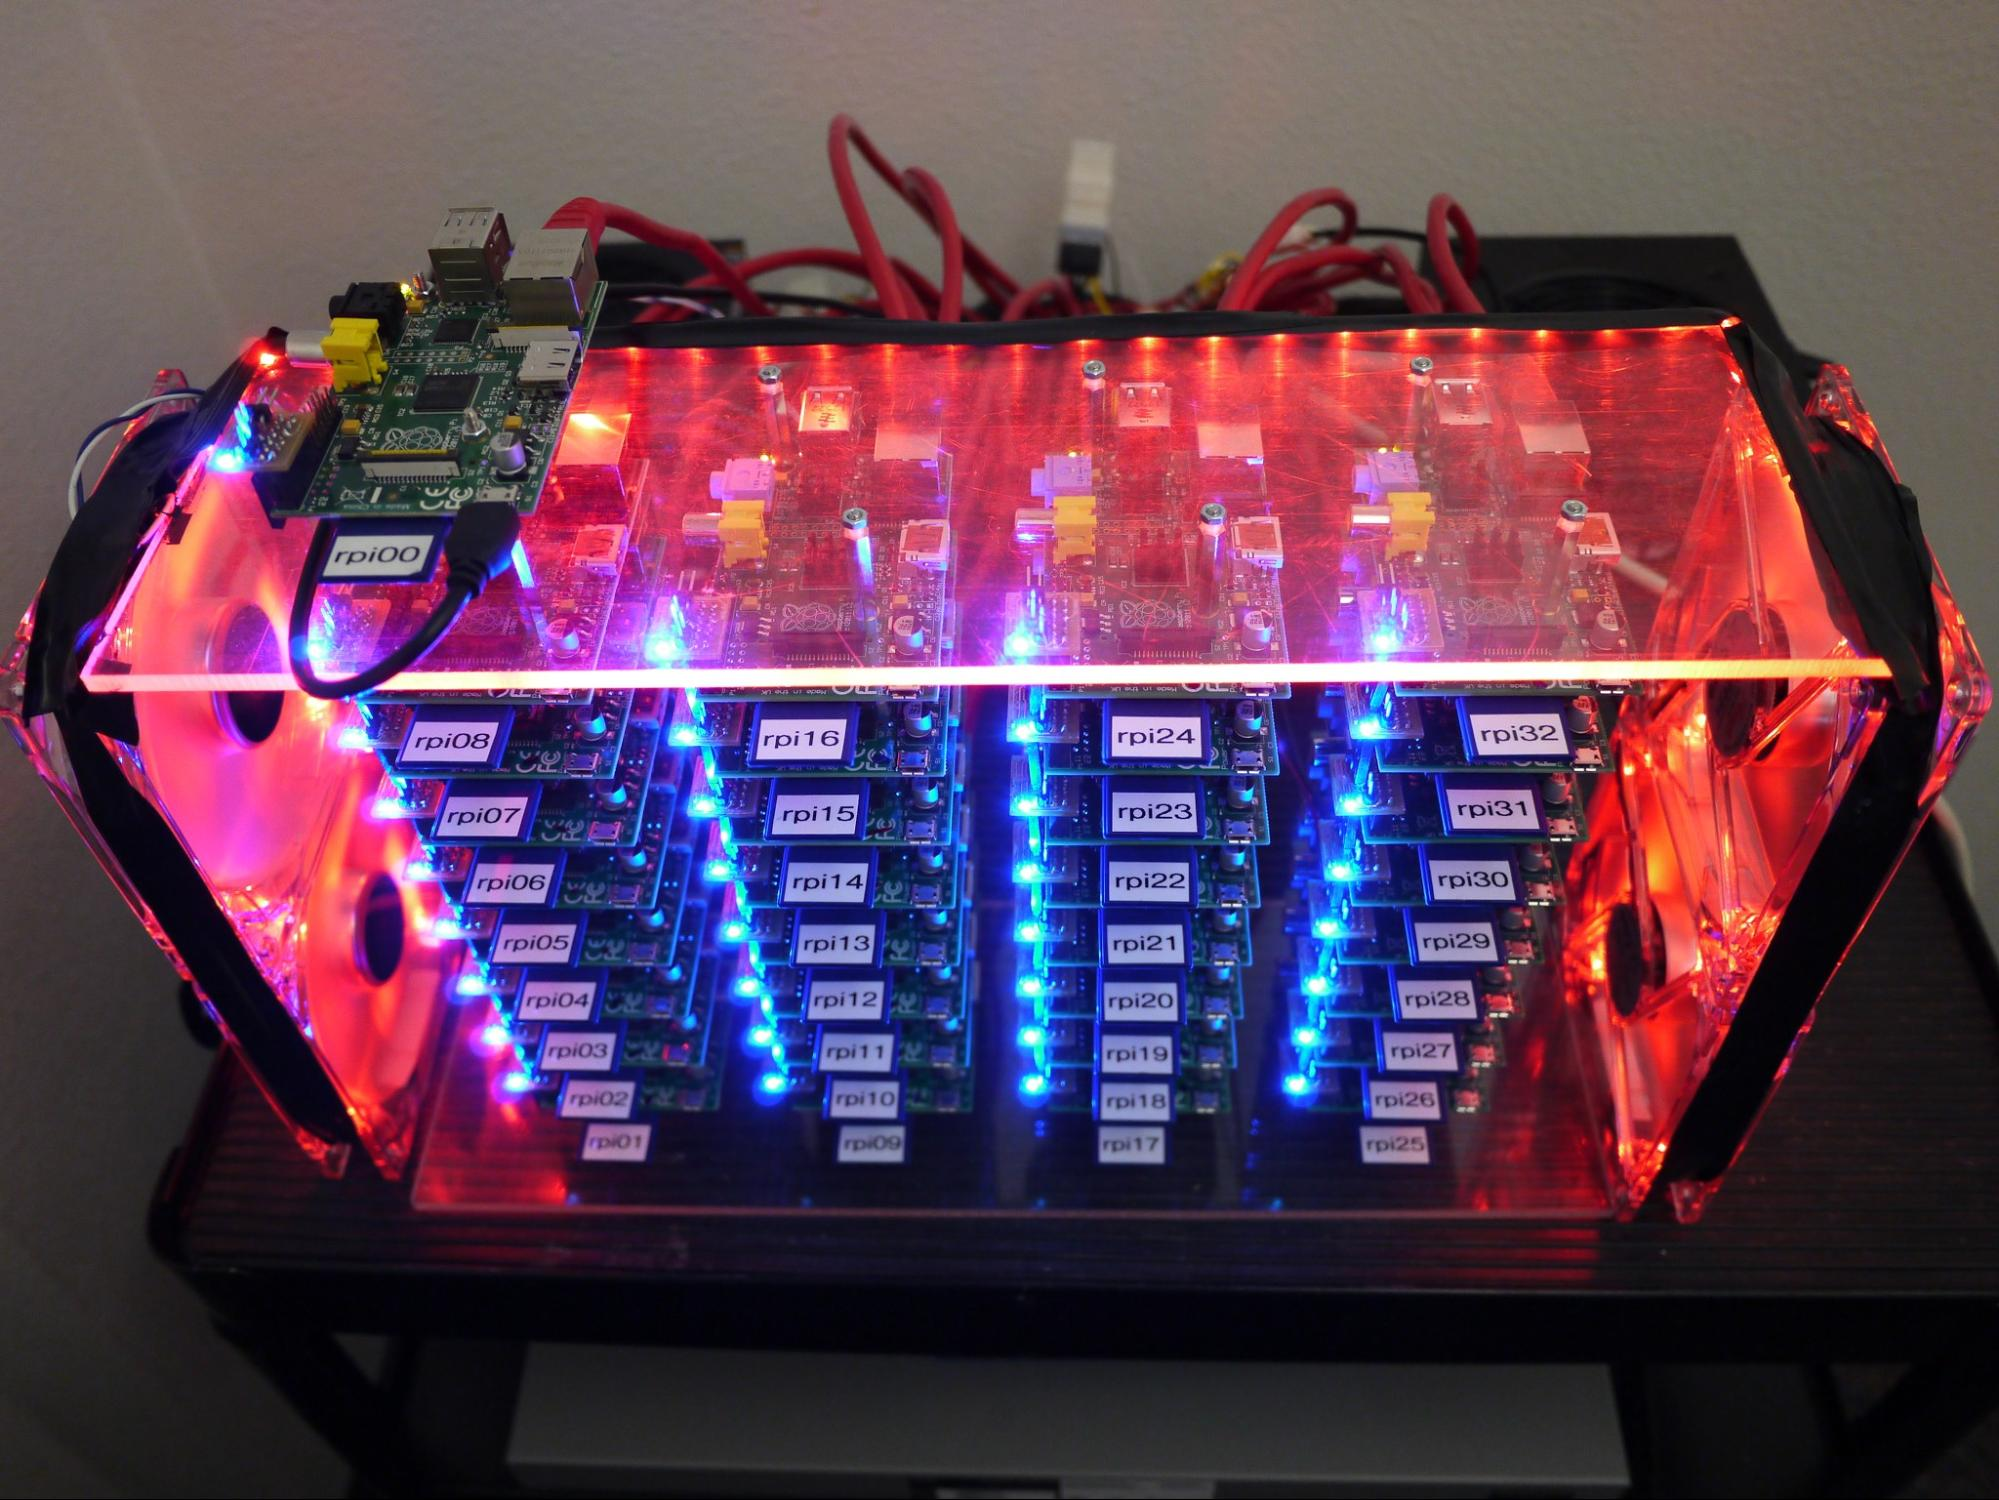
\includegraphics[width=0.36\textwidth]{Chapter3/Figures/kiepert-main}
  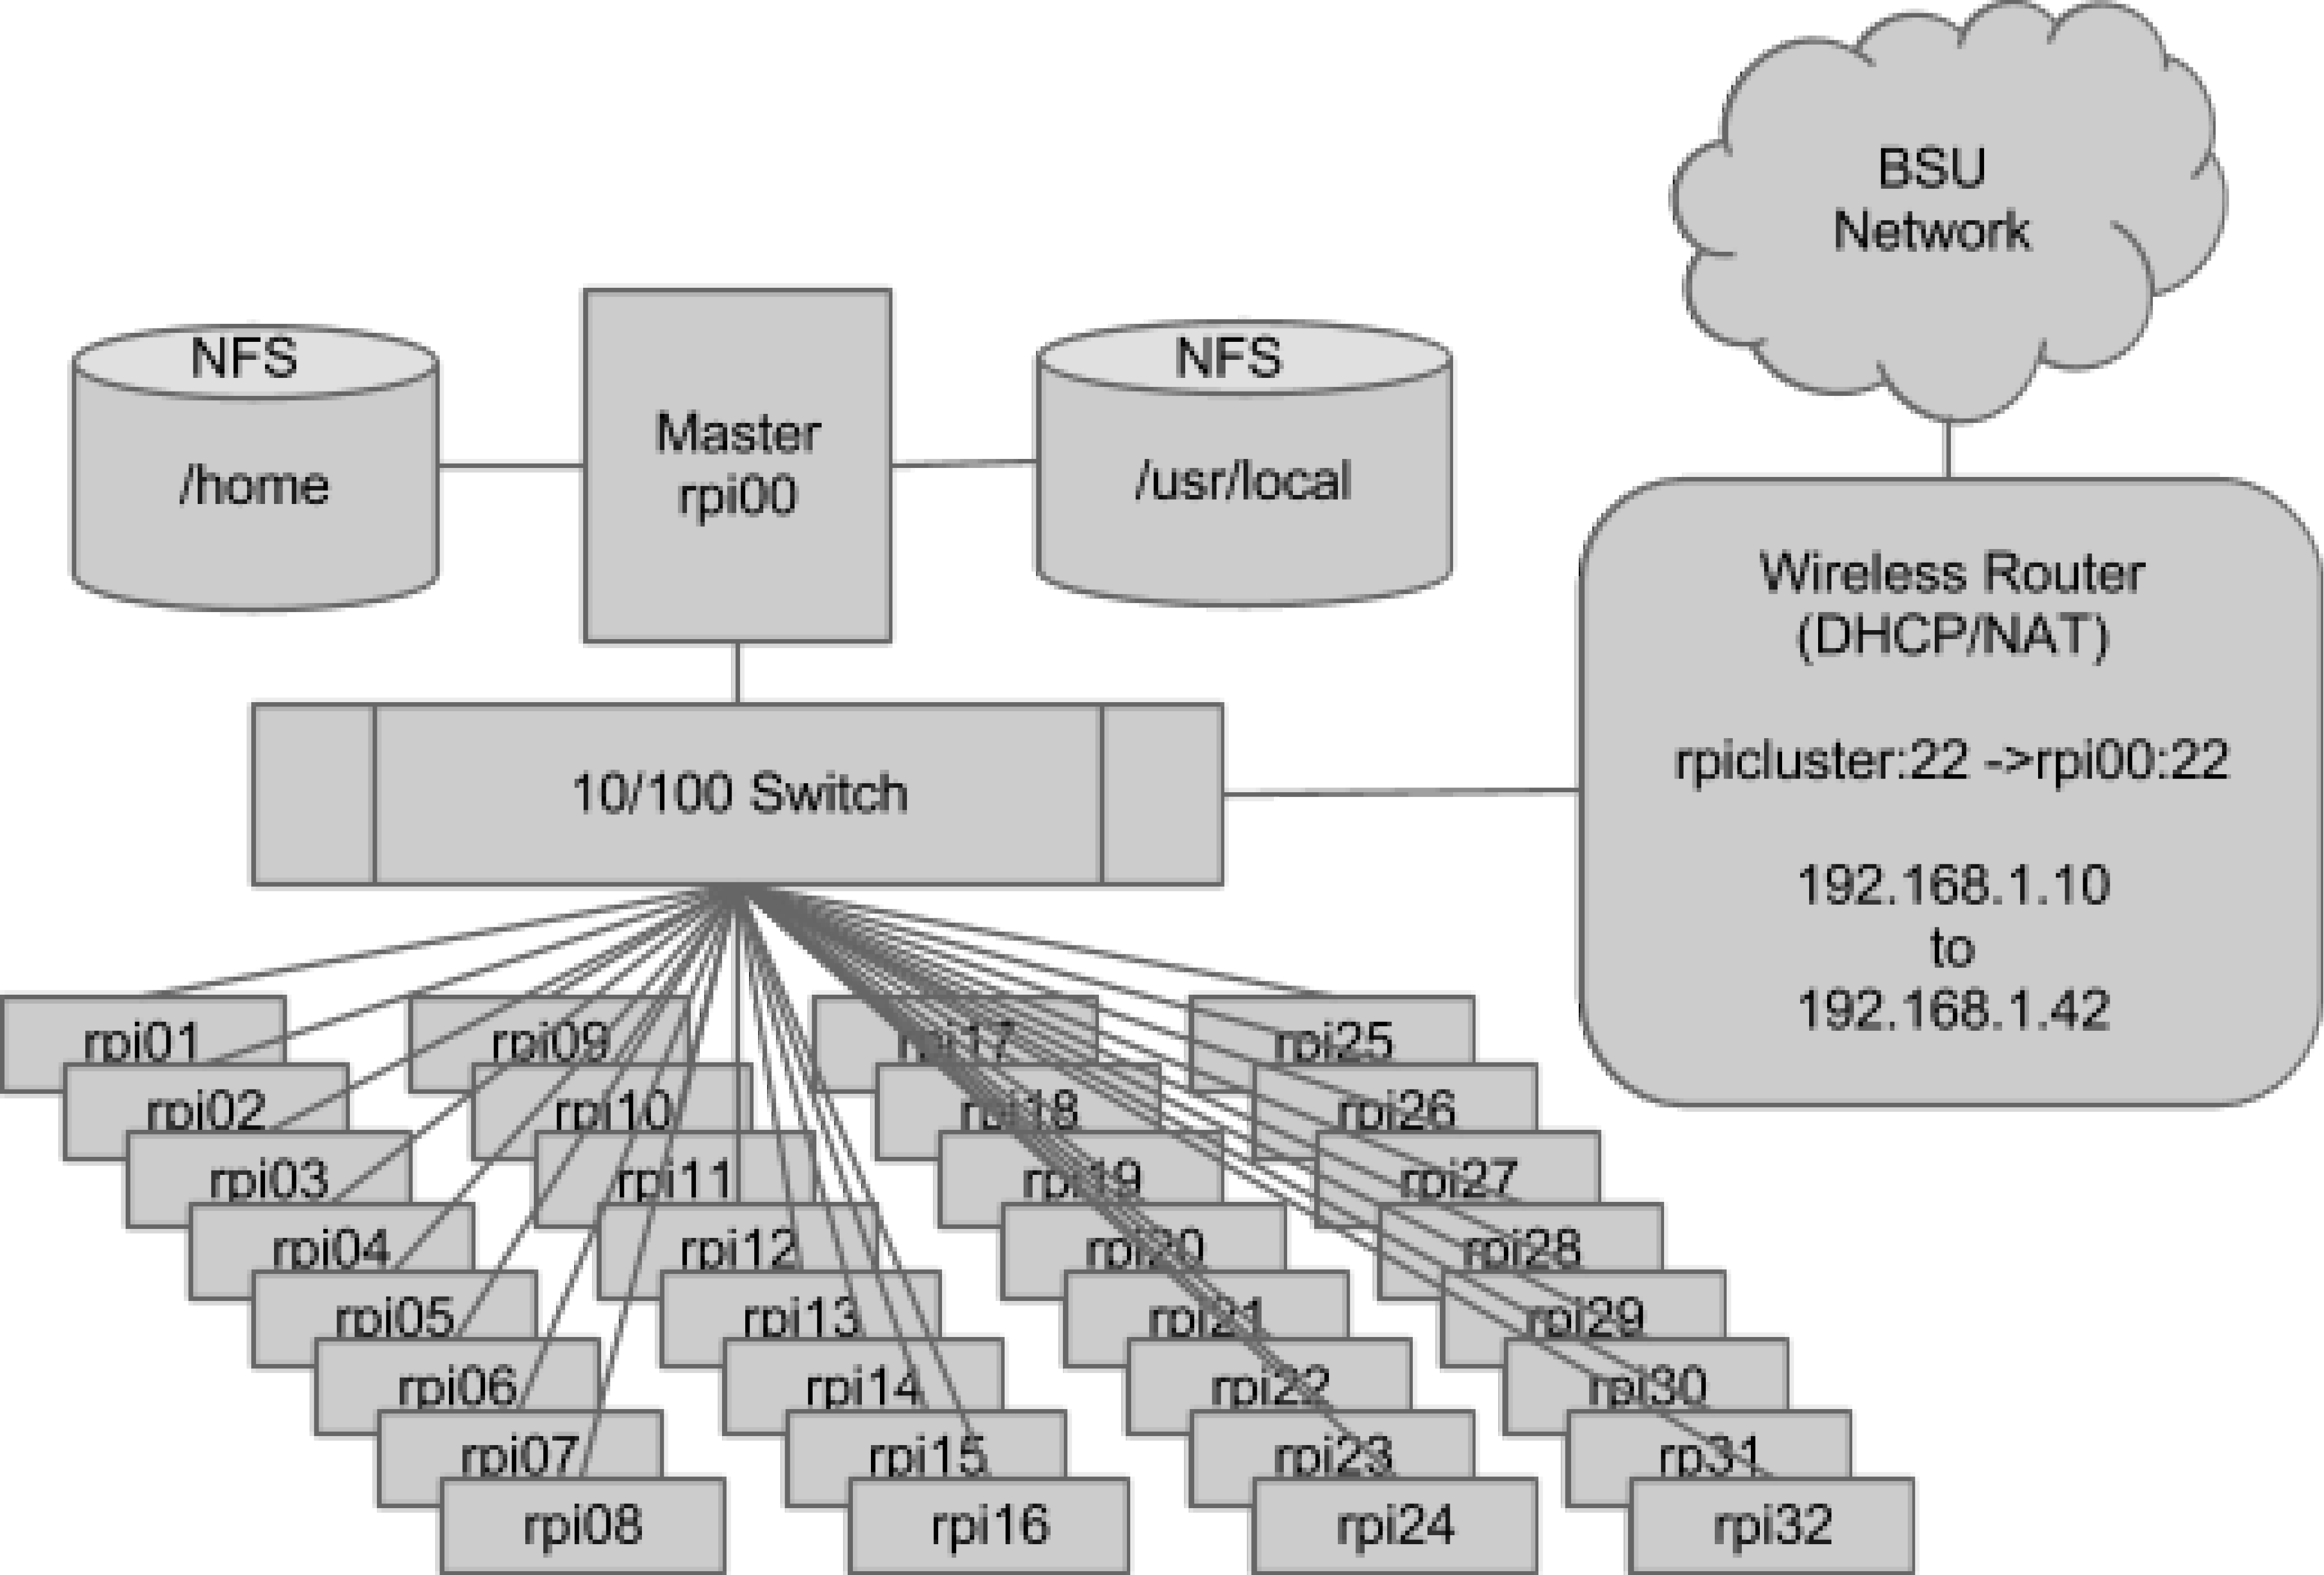
\includegraphics[width=0.4\textwidth]{Chapter3/Figures/kiepert.png}
  \caption[RPiCluster]{Vista general y estructura del sistema (Fuente: Joshua Kiepert)}
  \label{kiepert:structure}
\end{figure}

El coste total del proyecto según Kiepert es de 1967.21 dólares.

\subsubsection{Dramble (Jeff Geerling)}

El clúster \textit{Dramble} está formado por 6 equipos \textbf{Raspberry Pi} capaces de ejecutar en conjunto el gestor de contenidos \textbf{Drupal}\footnote{\href{https://www.drupal.org/}{drupal.org}}. Es utilizado como servidor de pruebas para la ejecución de instancias de este \textit{software} de forma experimental o durante demostraciones en público\cite{geerlingraspberry}. Se compone del conjunto de nodos \textit{Rasbperry Pi} y los mecanismos de red y alimentación que interconectan y proveen de energía a los mismos.

\begin{figure}[H]
  \centering
  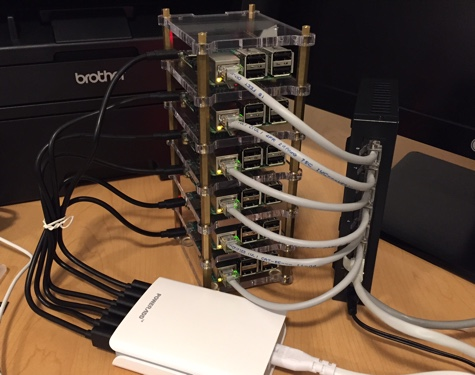
\includegraphics[width=0.5\textwidth]{Chapters/Chapter3/Figures/raspberry-pi-dramble-cluster-wired.jpg}
  \caption[Dramble]{El \textit{Dramble} en ejecución}
  \label{geerling:dramble}
\end{figure}

El coste estimado es de 35 dólares por cada Raspberry Pi mas el coste añadido de la red y el cableado de alimentación, totalizando aproximadamente 300 dólares.

\subsection{Bramble (GCHQ)}

El organismo gubernamental \textit{Government Communication Headquarters}, agencia de inteligencia del Gobierno Británico presentó en la \textit{Big Bang Fair} de 2015 un proyecto educativo que combina 66 \textit{Raspberry Pi} en un clúster jerárquico con 8 grupos de 8 nodos, cada uno de ellos con un coordinador. El cableado se reduce gracias al uso de la tecnología \textbf{PoE} (\textit{Power over Ethernet}), y cada \textbf{Raspberry} cuenta con un conjunto de elementos adicionales, como un reloj de tiempo real, disco duro externo, cámara, o punto de acceso WiFi\cite{gchqbramble}.

\begin{figure}[H]
  \centering
  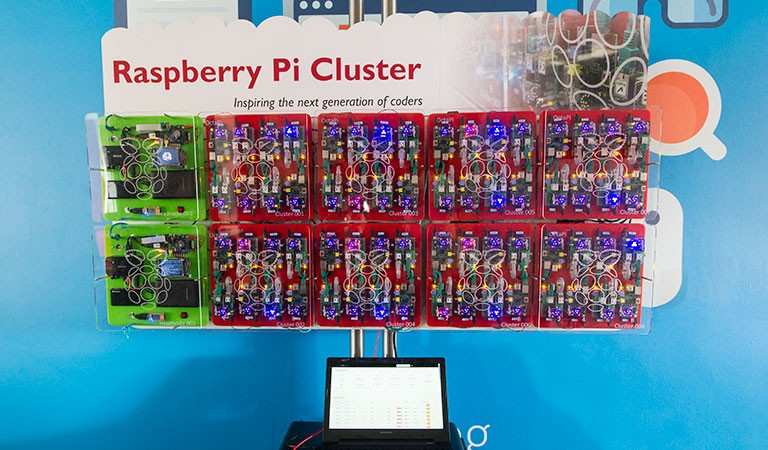
\includegraphics[width=0.8\textwidth]{Chapters/Chapter3/Figures/bramblegchq}
  \caption[Bramble]{Vistazo general de la estructura del sistema Bramble}
  \label{gchq:bramble}
\end{figure}

Se desconocen datos sobre el coste total del sistema.

\subsection{Clúster Iridis (Simon Cox, University of Southampton)}

Con el objetivo de atraer a jóvenes estudiantes al mundo de la computación, el profesor Simon Cox crea este clúster con 64 \textbf{Raspberry Pi B} sobre una estructura construida con LEGO\cite{cox:raspberry}. El sistema está diseñado para ejecutar aplicaciones sobre \textit{MPI}. Se desconocen datos sobre el coste total del sistema.

\begin{figure}[H]
  \centering
  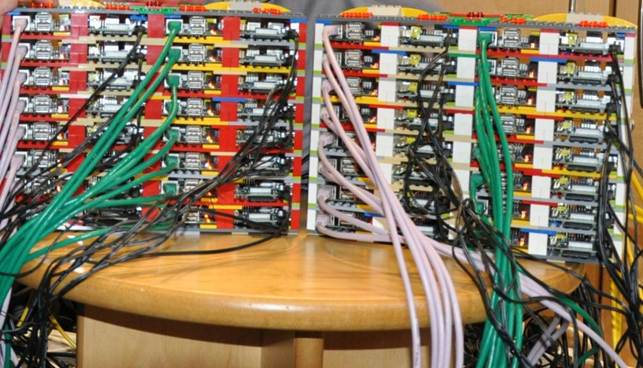
\includegraphics[width=0.65\textwidth]{Chapters/Chapter3/Figures/iridis-pi.jpg}
  \caption[Iridis]{Clúster Iridis}
  \label{cox:iridis}
\end{figure}

\subsection{Paralella}

Paralella es un proyecto de la compañía Adapteva que integra en un único chip un conjunto elevado de procesadores independientes con el objetivo de incrementar la capacidad de procesamiento total del sistema a un coste muy reducido\cite{paralella}. El coste es de 99 dólares por unidad.

\subsection{Virtualización}

Uno de los mecanismos para crear sistemas distribuidos en auge es la utilización de mecanismos de virtualización (ver \ref{teoria:virtualizacion}, que evitan el uso de diferentes unidades de \textit{hardware}. Estas soluciones se han popularizado en los últimos años principalmente en entornos empresariales, existiendo gran cantidad de proveedores de servicios y herramientas para la creación de un sistema propio (ver \ref{teoria:virtualizacion}). Ejemplos de este tipo de proveedores son \textbf{Amazon Web Services}\footnote{\href{http://aws.amazon.com/}{https://aws.amazon.com}}, \textbf{Google App Engine}\footnote{\href{https://cloud.google.com/appengine/}{https://cloud.google.com/appengine/}}, \textbf{Microsoft Azure}\footnote{\href{http://azure.microsoft.com/}{http://azure.microsoft.com/en-us/}} o \textbf{Digital Ocean}\footnote{\href{http://digitalocean.com}{http://digitalocean.com}}, entre muchos otros. Su éxito reside en su gran versatilidad: es sencillo crear y destruir nuevas réplicas de un sistema bajo demanda, ahorrando costes de forma significativa.

\subsection{\textit{Commercial Off-The-Shelf hardware}}

Este tipo de hardware está constituido por equipos disponibles al público de forma inmediata (\textit{off the shelf}) y generalmente son máquinas de propósito general, las cuales son interconectadas para crear un sistema distribuido que sirva de alternativa a utilidades más potentes, pero de coste superior (como un \textit{mainframe} o un ordenador de mayor potencia). Su coste económico (que se reduce si existe la posibilidad de aprovechar \textit{hardware} existente en la organización, como equipos de escritorio que no están en uso) es su mayor atractivo.

Un ejemplo de este tipo de sistemas son los clústeres \textit{Beowulf}\cite{beowulf:icpp95}, que se construyen sobre una red de área local y un sistema de intercomunicación como \textbf{MPI}, \textbf{PVM} u \textbf{OpenMP}. Existe gran cantidad de documentación para la creación de un clúster de este tipo\footnote{\href{http://tldp.org/HOWTO/Beowulf-HOWTO/}{tldp.org/HOWTO/Beowulf-HOWTO/}}, así como una serie de recursos (sistemas operativos, herramientas\dots) diseñadas con el propósito específico de crear este tipo de sistemas.


\section{Evaluación de alternativas}
\label{alternativas}
A la hora de evaluar las diferentes opciones que satisfagan los requisitos descritos, se consideran los siguientes aspectos:

\begin{itemize}
  \item Coste económico.
  \item Prestaciones técnicas (potencia de procesamiento, entrada/salida, capacidad de almacenamiento,facilidad de interconexión con otros elementos\dots).
  \item Facilidad de trabajo y de aprendizaje (documentación disponible, proyectos similares ya realizados, conocimiento previo sobre la plataforma en cuestión\dots).
  \item Escalabilidad del sistema.
  \item Necesidades de mantenimiento del sistema.
  \item Consumo eléctrico.
  \item Obsolescencia del sistema (periodo de tiempo en el que el \textit{hardware} y \textit{software} del sistema podrán ser actualizados y ser capaces de satisfacer los requisitos para los que fue creado).
\end{itemize}

\subsection{Propuesta de solución: Virtualización de entornos de trabajo}

Crear un conjunto de nodos virtuales dentro de una máquina que simulen un sistema distribuido

\paragraph{Ventajas intrínsecas de la solución\\}

Simplificación del sistema (reduce las necesidades de adquisición y mantenimiento de hardware).
Gestión de varias partes del sistema (sistema de ficheros centralizado, gestión de usuarios\dots) de forma mas sencilla. El coste se reduce significativamente.

\paragraph{Inconvenientes intrínsecos del sistema\\}

No se exploran apenas las posibilidades de un sistema distribuido formado por varios equipos físicamente independientes e impide aprovechar dicha independencia para los objetivos didácticos del sistema.

\paragraph{Facilidad de trabajo y curva de aprendizaje\\}

Si bien el trabajo con cada una de las instancias es previsiblemente sencillo, debido a la eliminación de la gran parte del mantenimiento de la capa física subyacente, el uso de este tipo de sistema requiere una etapa de formación previa en materia de virtualización.

\paragraph{Prestaciones técnicas\\}

Las prestaciones técnicas con las que se contaría, de llevarse a cabo este proyecto, son las de los equipos ya dispuestos para fines similares a este en el Centro\citationneeded[Preguntar a Andrés]{}.

\paragraph{Coste económico\\}

El coste económico es muy reducido si ya se cuenta con los equipos a utilizar y las licencias del \textit{software} de virtualización necesarias.

\paragraph{Escalabilidad del sistema\\}

Dependiente de las capacidades de virtualización del equipo disponible, y el número de nodos y usuarios a gestionar.

\paragraph{Necesidades de mantenimiento\\}

Las necesidades propias de un sistema operativo multiusuario (previsiblemente \textbf{GNU/Linux}) junto a las específicas de la virtualización de los equipos (monitor de máquinas virtuales).

\paragraph{Consumo energético del sistema\\}

\citationneeded[Preguntar a Andrés]{}

\paragraph{Obsolescencia del sistema\\}

Se estima una larga vida útil del sistema. Las máquinas virtuales instaladas en un sistema físico son fácilmente trasladables a otro equipo, por lo que la dependencia de la parte física del sistema es muy baja.

\paragraph{Material con el que se cuenta actualmente\\}

Se plantea el aprovechamiento de equipos ya presentes en la infraestructura en la que trabajar, por lo que se estima un coste muy pequeño a la hora de adquirir material.

\paragraph{Prestaciones técnicas\\}

\citationneeded[Preguntar a Andrés]{}

\paragraph{Análisis coste/beneficio\\}

Si bien el coste de esta solución es muy atractivo, presenta una serie de carencias que dificultan significativamente el desarrollo del sistema en el mismo. 


\subsection{Propuesta de solución: Clúster con equipos de escritorio}

Se plantea la reutilización de equipos de escritorio pertenecientes a la Universidad que ya no se encuentran en uso (debido a su renovación, falta de potencia como PC\dots) para la creación de este sistema.

\paragraph{Ventajas intrínsecas de la solución\\}

La potencia del sistema es mucho mayor que la de cualquier otra solución considerada. Se reduce dramáticamente el coste de adquisición de material y permite dar un nuevo ciclo de vida a material universitario. La arquitectura es conocida y fiable.

\paragraph{Inconvenientes intrínsecos del sistema\\}

No se exploran las características únicas de otros sistemas menos ``convencionales'', como los sistemas embebidos. El consumo energético es mayor y existe una mayor demanda de espacio que puede dificultar la implementación de diferentes aplicaciones didácticas ya planteadas como objetivo funcional del sistema.

\paragraph{Facilidad de trabajo y curva de aprendizaje\\}

Soporte completo de casi la totalidad de las distribuciones de GNU/Linux. Las necesidades de manipulación de hardware se minimizan.

\paragraph{Prestaciones técnicas}
\begin{itemize}
  \item Arquitectura x86/x86-64 (dependiendo de los equipos a utilizar finalmente).
  \item Entre 2 y 4 GB de memoria principal.
  \item Conectividad Ethernet, USB.
  \item Almacenamiento en disco duro.
\end{itemize}

\paragraph{Coste económico\\}

El coste económico de estos equipos es prácticamente nulo, pues ya se cuenta con los mismos y su utilización no exige la adquisición de nuevos equipos que los sustituyan. Estos equipos ya han sido retirados y no están empleados actualmente en ninguna tarea.

\paragraph{Escalabilidad del sistema\\}

Dependiente únicamente del coste económico de la adquisición de nuevos equipos, o de la disponibilidad de equipos que no estén utilizados.

\paragraph{Necesidades de mantenimiento\\}

Las propias de cualquier sistema multiusuario y las específicas del montaje dado (en materia de refrigeración, gestión de cableado, etcétera).

\paragraph{Consumo energético del sistema\\}

El típico de cualquier equipo de escritorio.

\paragraph{Obsolescencia del sistema\\}

Estos equipos tienen una antigüedad de aproximadamente 4 años. Dicha edad no impide que sean capaces de utilizar aplicaciones actuales, y en general no se prevé la incompatibilidad con ninguna aplicación. No obstante, son equipos relativamente antiguos que han sido utilizados de forma intensiva, por lo que la probabilidad de fallo en los mismos puede ser elevada.

\paragraph{Material con el que se cuenta actualmente\\}

Se cuenta con un número suficiente de equipos para la creación del sistema final.

\paragraph{Análisis coste/beneficio\\}

Si bien el coste de estos equipos es prácticamente nulo, dicho atractivo contrasta con los potenciales problemas que el uso de estos sistemas puede implicar (obsolescencia, uso de sistemas convencionales en detrimento de soluciones más innovadoras\dots).

\subsection{Clúster con equipos embebidos multimedia}

Utilización de equipos embebidos diseñados para aplicaciones multimedia en el sistema (ejemplos de alternativas comerciales son \textbf{Chromecast}, \textbf{Apple TV}, \textbf{Amazon Fire TV}\dots).

\paragraph{Ventajas intrínsecas de la solución\\}

Relación potencia/precio presumiblemente similar o superior a soluciones de coste similar como las placas Raspberry Pi.

\paragraph{Inconvenientes intrínsecos del sistema\\}

Dificultad de conexión (generalmente la conexión a red se realiza de forma inalámbrica, ausencia casi absoluta de cualquier conexión cuya finalidad no sea la emisión de contenido multimedia o la conexión con sistemas de almacenamiento), falta de puertos \textbf{GPIO}, \textbf{I\textsuperscript{2}C}\dots

\paragraph{Facilidad de trabajo y curva de aprendizaje\\}

Es difícil determinar la viabilidad de esta solución, pues no se cuenta con experiencia previa ni una documentación amplia al respecto. Además, es probable que sea necesaria la manipulación del sistema a muy bajo nivel, lo cual incrementa el grado de complejidad de la solución.

\paragraph{Prestaciones técnicas\\}

Como referencia se utilizan las prestaciones de uno de los equipos más populares, el \textbf{Google Chromecast}\footnote{\href{https://wikidevi.com/wiki/Google\_Chromecast\_\%28H2G2-42\%29}{https://wikidevi.com/wiki/Google\_Chromecast\_\%28H2G2-42\%29}}
\begin{itemize}
  \item Procesador ARM de 2 núcleos a 1.2 GHz.
  \item 512 MB de memoria principal.
  \item 2 GB de almacenamiento no extensibles.
  \item Alimentación por micro-USB.
  \item Utiliza un sistema operativo basado en \textbf{Google TV}, \textbf{ChromeOS} y \textbf{Android}.
\end{itemize}

\paragraph{Coste económico\\}

El coste de estos equipos es reducido, generalmente inferior a 30 € por unidad.

\paragraph{Escalabilidad del sistema\\}

Dependiente del coste de adquisición de nuevos equipos y las facilidades de interconexión de la plataforma (previsiblemente compleja, debido a la ausencia de sistemas de interconexión más allá de conexiones inalámbricas).

\paragraph{Necesidades de mantenimiento\\}

Dependiente del número de modificaciones que se realicen a las capas más bajas. En el peor de los casos puede que el administrador del sistema tenga que someterse a una etapa de formación para realizar un mantenimiento adecuado del sistema sin depender de los desarrolladores del mismo.
Otras necesidades son aquellas derivadas del mantenimiento de un sistema multiusuario sumadas a posibles problemas de interconexión si se utiliza una red inalámbrica (conexión a la LAN de la infraestructura local, interferencias\dots).

\paragraph{Consumo energético del sistema\\}

El diseño de estos equipos está orientado a la minimización del consumo energético, por lo que se estima reducido.

\paragraph{Obsolescencia del sistema\\}

La obsolescencia del sistema es difícil de determinar: no se cuenta con una gran cantidad de \textit{software} para este tipo de sistemas más allá de las aplicaciones multimedia.%TODO No obstante, el sistema subyacente es conocido (Linux).

\paragraph{Material con el que se cuenta actualmente\\}

No se dispone de material de estas o similares características.

% \subsection{Clúster con equipos embebidos multimedia\\}

% Utilización de equipos embebidos diseñados para aplicaciones multimedia en el sistema (ejemplos son Chromecast, Apple TV, Amazon Fire TV\dots)

% \paragraph{Ventajas intrínsecas de la solución}

% Relación potencia/precio presumiblemente superior a soluciones de coste similar como las placas Raspberry Pi.

% \paragraph{Inconvenientes intrínsecos del sistema}

% Dificultad de conexión (generalmente la conexión a red se realiza de forma inalámbrica, ausencia casi absoluta de cualquier conexión cuya finalidad no sea la emisión de vídeo o conexión con sistemas de almacenamiento mediante USB), falta de puertos GPIO, I2C\dots

% \paragraph{Facilidad de trabajo y curva de aprendizaje}
% Es difícil determinar la viabilidad de esta solución, pues no se cuenta con experiencia previa ni una documentación amplia al respecto.
% Es probable que sea necesaria la manipulación del sistema a muy bajo nivel. Lo cual incrementa el grado de complejidad de la solución.

% \paragraph{Prestaciones técnicas}
% Arquitectura ARM
% 2 núcleos a 1.2 GHz
% 512 MB de RAM
% Almacenamiento: 2 GB no expandibles
% Alimentación por microUSB

% \paragraph{Coste económico}


% \paragraph{Escalabilidad del sistema}
% Dependiente del coste de adquisición de nuevos equipos y las facilidades de interconexión de la plataforma (previsiblemente compleja, debido a la ausencia de sistemas de interconexión más allá de WiFi)

% \paragraph{Necesidades de mantenimiento}

% Dependiente del número de modificaciones que se realicen a las capas más bajas. En el peor de los casos puede que el administrador del sistema tenga que someterse a una etapa de formación para realizar un mantenimiento adecuado del sistema sin depender de desarrolladores previos.
% Las derivadas del mantenimiento de un sistema Linux sumadas a posibles problemas de interconexión si se utiliza una red inalámbrica (conexión a  la LAN de la infraestructura local, interferencias\dots).

% \paragraph{Consumo energético del sistema}


% \paragraph{Obsolescencia del sistema}

% Difícil de determinar: no se cuenta con una gran cantidad de software para este tipo de sistemas más allá de las aplicaciones multimedia. No obstante, el sistema subyacente es conocido (Linux)

% \paragraph{Material con el que se cuenta actualmente}

% No se dispone de material de estas o similares características

% \paragraph{Otras características}

\subsection{Clúster con sistemas embebidos}

Recientemente han surgido en el mercado sistemas embebidos con capacidad de cómputo elevada y precio muy reducido (en torno a los 40 euros por unidad). Estos equipos destacan además por su versatilidad. La mayoría de ellos son capaces de ejecutar una gran variedad de sistemas operativos (GNU/Linux, RISC OS, BSD, Windows\dots), incluyen una gran cantidad de mecanismos de interconexión y soportan la mayoría de herramientas presentes en equipos de escritorio y servidores.

Se plantea utilizar este tipo de plataformas para la creación del sistema, disponiendo los diferentes equipos en un pequeño ``rack'' con un sistema de alimentación propio centralizado y una conexión directa a la infraestructura local.

\paragraph{Ventajas intrínsecas de la solución\\}

Existen varias soluciones similares bien documentadas.
El hardware es flexible, barato y el consumo es pequeño.
Gran comunidad de desarrolladores alrededor de la plataforma.

\paragraph{Inconvenientes intrínsecos del sistema\\}

La potencia del sistema es pequeña.

\paragraph{Facilidad de trabajo y curva de aprendizaje\\}

Existe una amplia documentación del \textit{hardware} de este tipo de equipos, así como numerosos proyectos basados en los mismos, entre los que se incluyen sistemas similares a la solución planteada. Se cuenta además con experiencia en el manejo de estas placas.

\paragraph{Prestaciones técnicas}

\begin{itemize}
  \item Generalmente basados en la arquitectura ARM.
  \item Entre 512 MB y 2 GB de memoria principal.
  \item Conectividad \textbf{Ethernet},\textbf{I\textsuperscript{2}C}, \textbf{GPIO}, \textbf{USB}.
  \item Alimentación a través de \textbf{USB}/\textbf{GPIO}.
  \item Almacenamiento secundario basado en tarjetas microSD/SD, expansible a través de USB.
\end{itemize}

\paragraph{Coste económico\\}

Muy reducido, con un coste por nodo de entre 20 y 40 euros, al que se debe añadir los mecanismos de alimentación e interconexión.

\paragraph{Escalabilidad del sistema\\}

Dependiente únicamente del coste económico de la adquisición de nuevos equipos.

\paragraph{Necesidades de mantenimiento\\}

Las mismas que cualquier sistema multiusuario.

\paragraph{Consumo energético del sistema\\}

Variable según modelo, entre 3 y 4 W, con 5V de tensión y un amperaje variable entre 0.6 y 0.8 A.

\paragraph{Obsolescencia del sistema\\}

El software de terceros (sistema operativo, bibliotecas, etc) a incluir está respaldado por una comunidad extensa que provee actualizaciones de forma continua, por lo que previsiblemente el sistema podrá estar actualizado durante varios años.
Se prevé que las necesidades que el sistema cubre no demandarán una mayor potencia de cálculo en el futuro.

\paragraph{Material con el que se cuenta actualmente\\}

El Departamento de Informática y Automática cuenta con varios de estos equipos actualmente que podrían disponerse para el uso en el proyecto.

\subsection{Elección de la solución}

Basándose en las características descritas anteriormente, se elige realizar el sistema utilizando sistemas embebidos de bajo coste en virtud de los siguientes aspectos positivos:

\begin{itemize}
\item Compatibilidad con de gran cantidad de \textit{software} y sistemas operativos.
\item Versatilidad y facilidad de interconexión.
\item Se cuenta con experiencia en el uso de este tipo de dispositivos.
\item Bajo coste.
\end{itemize}

%TODO: Análisis de diferentes alternativas

\subsection{Raspberry Pi: Elección de las características básicas del sistema}

Se opta por las placas de la familia \textbf{Raspberry Pi} para la realización el sistema debido a la gran cantidad de soporte con el que cuentan, tanto por parte de la fundación \textbf{Raspberry Pi} como por diferentes comunidades de desarrolladores. Es el computador de este tipo que más sistemas operativos soporta\footnote{\href{http://elinux.org/RPi_Distributions}{http://elinux.org/RPi\_Distributions}} y existen gran cantidad de proyectos que dotan de mayor funcionalidad al sistema y que generalmente son diseñados para aprovechar las características del \textit{hardware} específico de la máquina.

Comparativa de las características relevantes de los diferentes modelos de Raspberry Pi.
Quedan descartados los modelos A y A+ por la carencia de puerto Ethernet (amén de otras características necesarias).
\begin{landscape}
\begin{table}[h]
\begin{tabular}{|p{3.2cm}|p{6cm}|p{6cm}|p{6cm}|}
\hline
 & \textbf{Modelo B} & \textbf{Modelo B+} & \textbf{Modelo B 2}\\ \hline
\textbf{Procesador} & ARMv6 1 Núcleo, 700 MHz (safe overclock hasta 1GHz) & ARMv6 1 Núcleo, 700 MHz (safe overclock hasta 1GHz) & ARMv7 4 Núcleos a 900 MHz \\ \hline
\textbf{Memoria} & 512 MB compartidos con GPU & 512 MB compartidos con GPU & 1 GB compartido con GPU\\ \hline
\textbf{LINPACK} \cite{hackaday:benchmarkpi2,gist:linpackbenchmark,elinux:benchmark} & 40.64 & 40.64 & 92.88\\ \hline
\textbf{Conexiones} & 2 USB, GPIO de 8 pines. Ethernet 10/100 & 4 USB, GPIO de 17 pines. Ethernet 10/100 & 4 USB, GPIO de 17 pines. Ethernet 10/100\\ \hline
\textbf{Consumo medio} & 700 mA, 5 V (3.5 W) & 600 mA, 5 V (3 W) & 800 mA, 5 V (4 W)\\ \hline
\textbf{Almacenamiento} & SD & microSD & microSD\\ \hline
\textbf{Alimentación} & Mediante micro-USB o los pines GPIO & Mediante micro-USB o los pines GPIO &Mediante micro-USB o los pines GPIO\\ \hline
\textbf{Sistemas operativos compatibles} & 

Arch Linux ARM, OpenELEC, Puppy Linux, Raspbmc, RISC OS, Raspbian, XBian, openSUSE, Slackware ARM, FreeBSD, Plan 9, Kali Linux, Sailfish OS, Pidora (Fedora Remix), Lista completa en \footnote{\href{http://elinux.org/RPi\_Distributions}{http://elinux.org/RPi\_Distributions}} & Los mismos que para el modelo B & Hasta la fecha, únicamente:

Ubuntu Snappy Core, Raspbian, OpenELEC, RISC OS, Según la web de Arch Linux, también soporta este sistema operativo \footnote{\href{http://archlinuxarm.org/platforms/armv7/broadcom/raspberry-pi-2}{archlinuxarm.org/platforms/armv7/broadcom/raspberry-pi-2}} \\

\hline % 

\textbf{Otros} & Modelo descatalogado, el soporte oficial y proporcionado por la comunidad probablemente será menor que para los modelos más recientes en el futuro. &  & Lleva poco tiempo en el mercado (apenas un mes). Se conocen pequeños fallos en el hardware (fotosensibilidad de algún componente).\\ \hline

\end{tabular}
\caption{Comparativa de los diferentes modelos de Raspberry Pi}
\end{table}
\end{landscape}

\citationneeded[https://learn.adafruit.com/embedded-linux-board-comparison/performance]
\citationneeded[https://learn.adafruit.com/introducing-the-raspberry-pi-2-model-b/performance-improvements]
\citationneeded[http://raspi.tv/2014/how-much-less-power-does-the-raspberry-pi-b-use-than-the-old-model-b]

\begin{landscape}
\subsection{Elección del sistema operativo}
\label{os:evaluation}
\begin{table}[h]
\begin{tabular}{|p{1.6cm}|p{5cm}|p{4cm}|p{3cm}|p{4cm}|p{4cm}|}
\hline
\textbf{Nombre} & \textbf{Enfoque} & \textbf{Características notables} & \textbf{Ventajas} & \textbf{Inconvenientes} & \textbf{Software disponible}\\ \hline
\textbf{Arch Linux} ARM & Distribución ligera centrada en el minimalismo y la disponibilidad de software novedoso. Requiere sin embargo que el usuario esté familiarizado con el sistema GNU/Linux antes de utilizarlo. & Muy optimizado con un ciclo de desarrollo que permite contar con software puntero en poco tiempo. & Eficiente, gran comunidad alrededor, relativamente sencillo de utilizar. & En ocasiones puede ser complejo su uso. Ya no se incluye en las distribuciones por defecto de la Fundación Raspberry Pi, lo cual puede suponer falta de soporte oficial. & 8700 paquetes disponibles en los repositorios oficiales, más pequeño que para otras distribuciones, si bien equiparable si se cuenta el \textbf{AUR} (\textit{Arch User Repository})\\ \hline

\textbf{Ubuntu Snappy Core} & Centrado en la facilidad de uso. & Es la distribución más popular (en equipos de escritorio) contando con gran cantidad de \textit{software} disponible & Fácil de configurar, gran cantidad de soporte & Recientemente portado a la Raspberry de forma intensiva.El rendimiento de Ubuntu suele ser menor al de otros sistemas operativos debido a la gran cantidad de paquetes incluidos por defecto. & Unos 40000\footnote{\href{https://launchpad.net/ubuntu/trusty/armhf}{https://launchpad.net/ubuntu/trusty/armhf}}\\ \hline 

\textbf{Raspbian} & Centrado en la estabilidad del sistema en detrimento de las últimas versiones de los componentes del sistema. & Es el sistema más utilizado en la plataforma Raspberry Pi. La fundación Raspberry Pi promociona su uso y la mayoría de los desarrolladores de la plataforma crean herramientas para este sistema. & Estable, gran cantidad de \textit{software} disponible, ya conocido. & La instalación básica del sistema incluye una gran cantidad de herramientas que consumen recursos del sistema de forma significativa. & Unos 20000\\ \hline
\end{tabular}
\caption{Comparativa de sistemas operativos (1)}
\end{table}
\end{landscape}

\begin{landscape}
\begin{table}[h]
\begin{tabular}{|p{2cm}|p{4cm}|p{5cm}|p{3cm}|p{4cm}|p{4cm}|}
\hline
\textbf{Nombre} & \textbf{Enfoque} & \textbf{Características notables} & \textbf{Ventajas} & \textbf{Inconvenientes} & \textbf{Software disponible}\\ \hline

\textbf{RISC OS} & Diseñado específicamente para la arquitectura ARM, aprovechando las posibilidades de dicha arquitectura al máximo. & Eficiente, basado en el RISC OS original, incluyendo características del mismo. Sistema monousuario con multitarea cooperativa (en contraste con multihilo o multitarea apropiativa). & Muy eficiente & No esta basado en un sistema conocido previamente. Relativamente desfasado en cuanto a la arquitectura del sistema operativo. El software suele ser programado en BBC BASIC (con el que no se cuenta experiencia). & No se conocen cifras\\ \hline

\textbf{Gentoo} & Diseñado para permitir la modificación del sistema al máximo nivel posible. Todo el \textit{software} es compilado en la máquina que lo instala, en lugar de utilizar ejecutables precompilados & Enfocado en la personalización. & Permite ser modificado de forma sencilla. & Poco soportado en Raspberry Pi. & \\ \hline

\textbf{Windows 10} & Diseñado para el paradigma del Internet de las Cosas, & Sencillo de utilizar, con soporte (previsiblemente) del \textit{framework} \textbf{.NET}. & Soporta con un conjunto de tecnologías conocidas no compatibles con ninguna otra alternativa. Si el soporte de \textbf{.NET} es ofrecido constituiría una ventaja clave.  & Aún no se encuentra disponible\cite{windows10raspberry}. Esta diseñado para un propósito especifico. No compatible con software para Linux de forma nativa. & No se conocen cifras\\ \hline

\end{tabular}
\caption{Comparativa de sistemas operativos (2)}
\end{table}
\end{landscape}


\section{Ingeniería de sistemas: propuesta de solución definitiva}

En esta sección se describen los aspectos a alto nivel sobre todos los componentes que se integrarán en el sistema final (tanto \textit{hardware} como \textit{software}), así como las relaciones entre los mismos. En función de la evaluación llevada a cabo se extraen las siguientes decisiones de diseño que conforman la propuesta de solución definitiva.



\subsection{\textit{Hardware}}

\subsubsection{Nodos}

Todo el sistema se construirá sobre placas \textbf{Raspberry Pi 2} debido a su alta versatilidad, gran potencia de cálculo, interfaces de comunicación, soporte por parte de las diferentes comunidades de desarrolladores y consumo eléctrico.

\subsubsection{Equipos auxiliares}

En caso de que sea necesario integrar algún nodo en el sistema se utilizarán equipos \textbf{COTS} en desuso presentes en la infraestructura. La utilización de este tipo de nodos se realizará siempre con carácter auxiliar (e.g. para ofrecer un servicio que sea difícil de soportar por los nodos principales).

\subsubsection{Interconexión física}

El sistema deberá interconectar los diferentes nodos utilizando la red presente en la infraestructura (basada en el protocolo IP). No obstante se plantea el uso de dispositivos de enrutado o conmutación como medida de mejora del rendimiento.

\subsubsection{Alimentación}

La alimentación del sistema deberá proceder de una única fuente, a fin de minimizar las cantidades de  cableado, transformadores u otro tipo de elementos.

\subsubsection{Estructura}

Se deberá diseñar una estructura propia que recoja todos los componentes del sistema, a fin de facilitar la instalación en su ubicación final.

\subsection{\textit{Software}}

\subsubsection{Sistema operativo}
\label{problema:sistemaoperativo}

El sistema operativo a utilizar será \textbf{Arch Linux ARM}, debido a la gran comunidad de soporte con la que cuenta, compatibilidad con la gran mayoría de componentes presentes en un sistema GNU/Linux y modelo arquitectónico que apuesta por la simplicidad, \textit{limpieza} y eficiencia del sistema.

Se partirá de la instalación base provista por el proyecto, debido a que incluye el conjunto más pequeño de herramientas con el que el sistema operativo es capaz de trabajar, incluyendo posteriormente aquellas herramientas necesarias para la construcción del sistema. Este enfoque evita la inclusión de paquetes innecesarios que afectarían negativamente al rendimiento de la solución final.

\subsubsection{Componentes del sistema operativo}

Se crearán un conjunto de componentes que se integrarán en el sistema operativo y podrán ser aprovechados por aplicaciones creadas por usuarios o por herramientas internas del propio sistema. Dichos servicios incluyen mecanismos de descubrimiento, coordinación, acuerdo, autoconfiguración de componentes o gestión de usuarios, entre otros.

\subsubsection{Interfaces de conexión entre componentes}

Aquellos servicios ofrecidos por el sistema operativo que sean aprovechables por los usuarios finales deberán ofrecer una interfaz de conexión con los mismos. Dicha interfaz deberá apoyarse en mecanismos de interconexión conocidos y deberá ofrecerse en el mayor número de plataformas y lenguajes de programación posible.

\subsubsection{Servicios}

El sistema se plantea como un conjunto de nodos que ofertan servicios consumibles por otros componentes del sistema o por terceras partes. Dichos servicios deberán contar con una serie de puntos de acceso claramente definidos que constituirán las interfaces de uso de dichos servicios.

\subsubsection{Instalación y mantenimiento}

El sistema final se compondrá de un conjunto elevado de nodos, por lo que se espera que la instalación y configuración de los mismos sea un proceso tedioso. A fin de minimizar dicha carga de trabajo se crearán herramientas que automaticen dichas etapas, idealmente, de forma completa.

\subsubsection{Herramientas de desarrollo a utilizar}

Se plantea el uso del lenguaje de programación Python\footnote{\href{http://www.python.org}{http://python.org}} como herramienta principal de desarrollo, debido a su potencia de cálculo y simplicidad, que permite crear aplicaciones que consuman pocos recursos (aspecto vital, máxime cuando se utilizará sobre un sistema con un \textit{hardware} poco potente) de forma sencilla y rápida. También se plantea el uso de los lenguajes de programación C y C++ para el desarrollo de herramientas a bajo nivel, así como herramientas web para el desarrollo de aplicaciones utilizadas por el usuario.

\section{Integración}

\section{Proceso}

La determinación del proceso de desarrollo del sistema influirá significativamente en la consecución de los diferentes objetivos del sistema.

Las particulares características cada proyecto propician la elección de un proceso u otro. En el caso concreto del proyecto en cuestión se deben considerar las siguientes características:

\begin{itemize}

\item No se cuenta con experiencia previa en la construcción de varios componentes cruciales del sistema. Serán necesarias etapas de aprendizaje y la tolerancia a decisiones erróneas deberá ser alta, permitiendo rectificar posteriormente.

\item El proyecto tiene un alto componente de experimentalidad: el sistema final será el resultado de los diferentes procesos de investigación y prueba de soluciones para cada uno de los problemas planteados. La incertidumbre es por tanto alta, y por ello la toma de decisiones debe ser reversible, a fin de poder cambiar el enfoque aplicado a un problema si se detecta que los resultados del mismo serán infructuosos. Dicha reversibilidad implica principalmente la capacidad de poder rectificar en un periodo de tiempo pequeño, debido principalmente a la restricción de tiempo que el proyecto incluye.

\item Es esperable que los requisitos definidos en las diferentes fases del proyecto deban ser modificados debido a la gran incertidumbre con la que se debe lidiar.

\end{itemize}

Es por todo ello que es necesaria la determinación de un proceso de desarrollo que deje espacio a etapas de aprendizaje y experimientación, así como la modificación de los diferentes requisitos preestablecidos. 

\subsection{Elección del proceso}

En virtud de las razones expuestas se opta por un proceso ágil apoyado sobre prototipos. 

Un prototipo es un componente \textit{software} que implementa un subconjunto de la funcionalidad del sistema final y es funcional. El desarrollo de prototipos permite realizar evaluaciones de la funcionalidad implementada de forma efectiva ahorrando costes y tiempo de desarrollo. En el caso concreto de este proyecto posibilitan la evaluación de una alternativa sobre el resto, así como la viabilidad de una solución sobre el resto. Se apuesta por un modelo de desarrollo de prototipos evolutivo\cite{10.1109/TSE.1975.6312870}, creando versiones funcionales que paulatinamente crezcan en complejidad. Este tipo de prototipado permite experimentar con una estrategia de desarrollo (probar un algoritmo, experimentar con un lenguaje de programación, aprovechar una biblioteca, \textit{framework}\dots) y analizar las ventajas e inconvenientes de la misma en poco tiempo, siendo posible desechar el prototipo en caso de que el camino elegido no satisfaga los requisitos planteados.

Los procesos ágiles suelen ser utilizados a la hora de realizar un proyecto en equipos pequeños en entornos cambiantes o con un grado de incertidumbre muy alto. Procesos ``tradicionales'', como el desarrollo \textit{en cascada} o el lineal no responden de forma dinámica a dichas propiedades, y su adaptabilidad es menor.

En el caso del presente proyecto, se opta por un proceso ágil basado en iteraciones de corta duración (entre 7 y 12 días) con una serie de objetivos definidos y producen una versión más avanzada de los prototipos. Debido a que el proyecto comprende el desarrollo de una serie de productos independientes que conforman un sistema (en contraste con un único producto monolítico final) es necesario paralelizar el desarrollo de todos los procesos a lo largo de las diferentes iteraciones, balanceando la carga de trabajo entre las diferentes tareas.

\subsection{Desarrollo de subsistemas}
Los diferentes aspectos relativos al desarrollo de cada uno de los subsistemas se definen en los anexos dispuestos a tal efecto.

\subsection{Integración del sistema}

Se ha realizado un proceso de integración creciente de los diferentes prototipos creados como resultado de cada uno de los ciclos de desarrollo. Esta práctica es de utilidad para detectar diferentes fallos en el sistema o anomalías fruto de las interacciones entre componentes de forma temprana.

\subsection{Instalación del sistema}

Se han creado herramientas que facilitan la instalación del sistema (ver \ref{marcobootstrap}) en diferentes tipos de infraestructuras que cuenten con una serie de propiedades mínimas (conexión de red).
\citationneeded[Instalación del sistema físico: diferencias con el entorno de desarrollo, oposición de los usuarios, problemas de espacio físico]
\subsection{Evolución del sistema}

La solución presentada es altamente escalable y existe un equipo de soporte para todos los componentes el \textit{software} utilizado, aspetos que garantizan la inclusión de nuevas características y el mantenimiento de los paquetes instalados.  

\subsection{Desmantelamiento del sistema}

Ningún componente contiene materiales cuya manipulación incorrecta pueda dañar su entorno. En el caso de que el desmantelamiento no se produzca por fallos en el \textit{hardware} del sistema, sus componentes pueden ser aprovechados para otros proyectos académicos o profesionales por su poseedor. Los diferentes paquetes \textit{software} no dependen del hardware del sistema para funcionar, salvo varias exceptiones, tales como herramientas creadas para un problema concreto de esta plataforma\footnote{Como Marcobootstrap, entre otros}.

%TODO: IS 1 T2 Pg 34
Fases
\begin{itemize}
  \item Definición de requisitos
  \item Diseño
\end{itemize}

%Proceso unificado ágil
%https://en.wikipedia.org/wiki/Scrum_%28software_development%29
%https://en.wikipedia.org/wiki/Extreme_programming
%https://en.wikipedia.org/wiki/Crystal_Clear_%28software_development%29


%\section{Desarrollo}

%REDMINE-driven description